% Provenance (never printed): cycle 2 "Questionner le monde" (states of water in
% weather phenomena; daily observation), see sources/book1/PROVENANCE.md.
% Book 1, grade 1, chapter 1. No real-world number in this chapter.
\chapter{Observer le temps qu'il fait}\label{ch:g1:watching-the-weather}

Il est tôt le matin. Lena se réveille, grimpe sur la chaise près de la
fenêtre de sa chambre et regarde dehors. Le ciel est gris. De petites
gouttes d'eau coulent sur la vitre. Les toits d'en face sont mouillés et
brillants, et l'arbre du jardin s'égoutte.

«~Qu'est-ce que je vais mettre aujourd'hui~?~» demande-t-elle.

Pour répondre, Lena n'a besoin ni d'un livre ni d'une machine. Il lui
suffit de regarder par la fenêtre. La fenêtre est sa première station \omterm{def:g1:watching-the-weather:weather}{météo}.

\begin{omfigure}
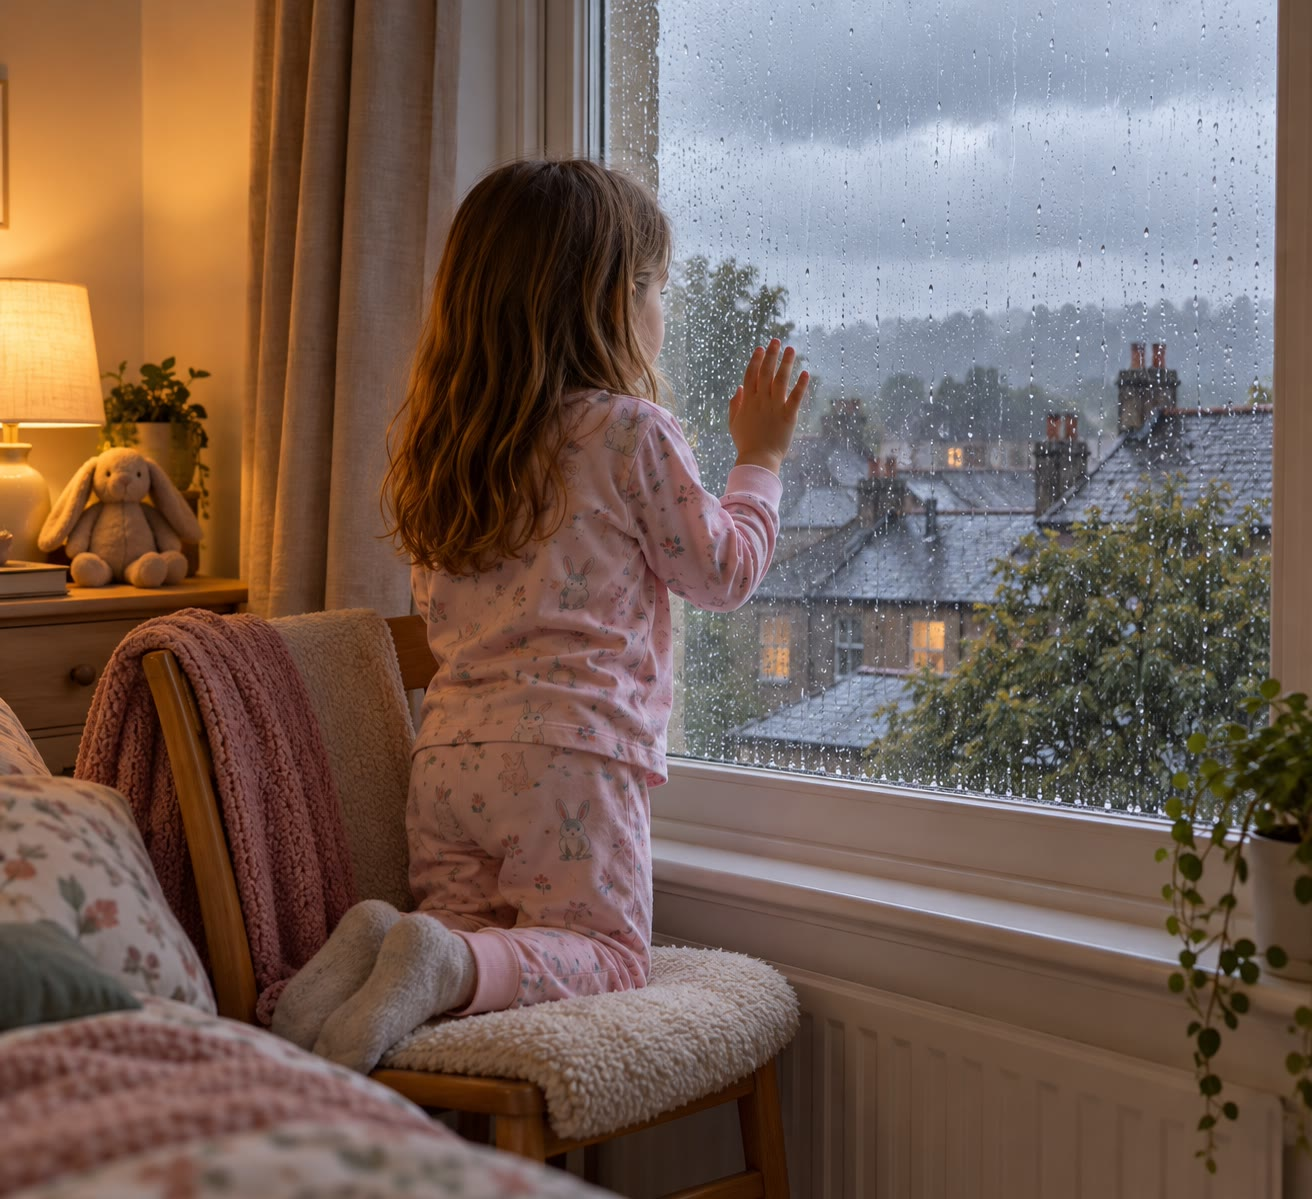
\includegraphics[width=0.72\linewidth]{images/book1/ai/g1-rainy-window.jpg}

{\small Un matin gris et pluvieux, vu à travers une fenêtre.}
\end{omfigure}

\begin{recall}
Chaque matin, le Soleil se lève et le jour commence~; chaque soir, il se
couche et la nuit arrive. Dans les livres de physique, tu as vu pourquoi la
nuit succède au jour. Dans ce chapitre, nous regardons autre chose qui
change tout le temps~: le \omterm{def:g1:watching-the-weather:weather}{temps qu'il fait}.
\end{recall}

\section{Quel temps fait-il~?}

Quand nous sortons, nous sentons l'air sur notre visage. Il peut être doux
ou froid. Il peut être immobile, ou bien pousser nos cheveux et nos
vêtements~: alors il y a du vent. Nous levons les yeux vers le ciel. Il
peut être bleu et lumineux, ou couvert de nuages. Parfois la pluie tombe
des nuages, parfois la neige. Tout cela ensemble, c'est le \omterm{def:g1:watching-the-weather:weather}{temps qu'il fait}.

\begin{definition}[Le temps qu'il fait]\label{def:g1:watching-the-weather:weather}
Le \emph{temps qu'il fait}\index{temps qu'il fait}, c'est l'état de l'air et
du ciel en un lieu et à un moment donnés~: ensoleillé ou nuageux, sec,
pluvieux ou neigeux, calme ou venteux, chaud ou froid.
\end{definition}

Pour décrire le \omterm{def:g1:watching-the-weather:weather}{temps qu'il fait}, nous répondons à quelques questions simples~:
\begin{enumerate}
  \item \textbf{À quoi ressemble le ciel~?} Est-il bleu, avec le Soleil
        qui brille~? Y a-t-il quelques nuages, ou le ciel est-il tout gris~?
  \item \textbf{Quelque chose tombe-t-il du ciel~?} De la pluie~? De la
        neige~? Rien~?
  \item \textbf{Y a-t-il du vent~?} Les feuilles des arbres bougent-elles~?
        Un drapeau claque-t-il~?
  \item \textbf{Fait-il chaud ou froid~?} Avons-nous besoin d'un manteau~?
\end{enumerate}

\begin{omfigure}
\begin{minipage}[b]{0.49\linewidth}\centering
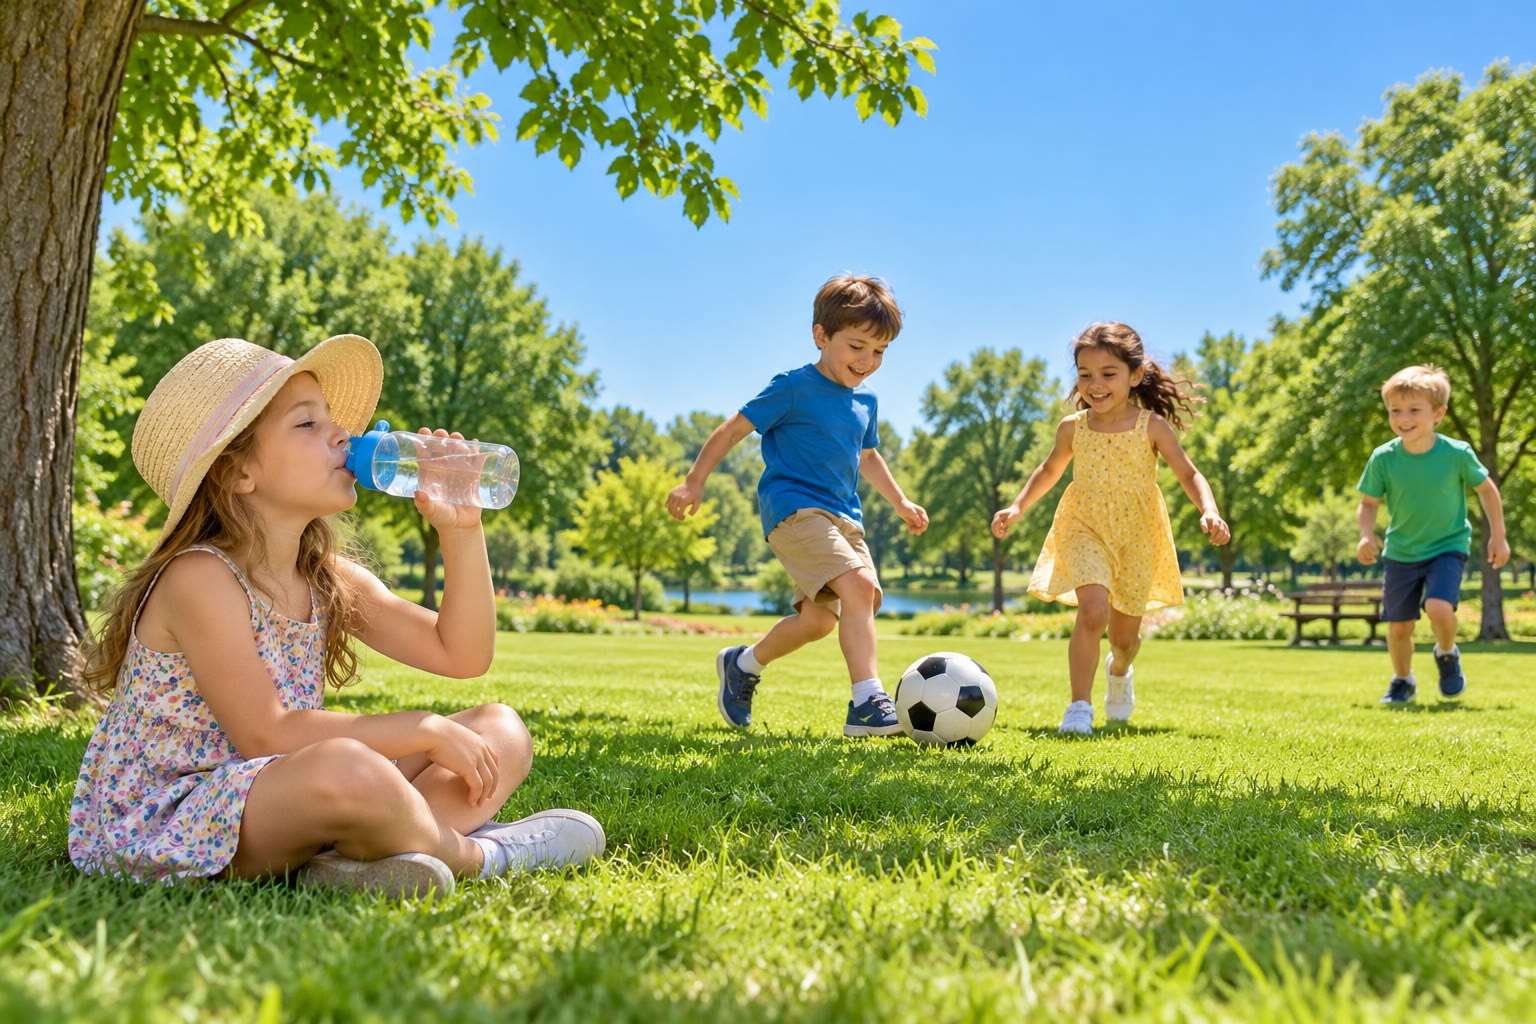
\includegraphics[width=\linewidth]{images/book1/ai/g1-sunny-park.jpg}

{\small Du soleil, et il fait chaud.}
\end{minipage}\hfill
\begin{minipage}[b]{0.49\linewidth}\centering
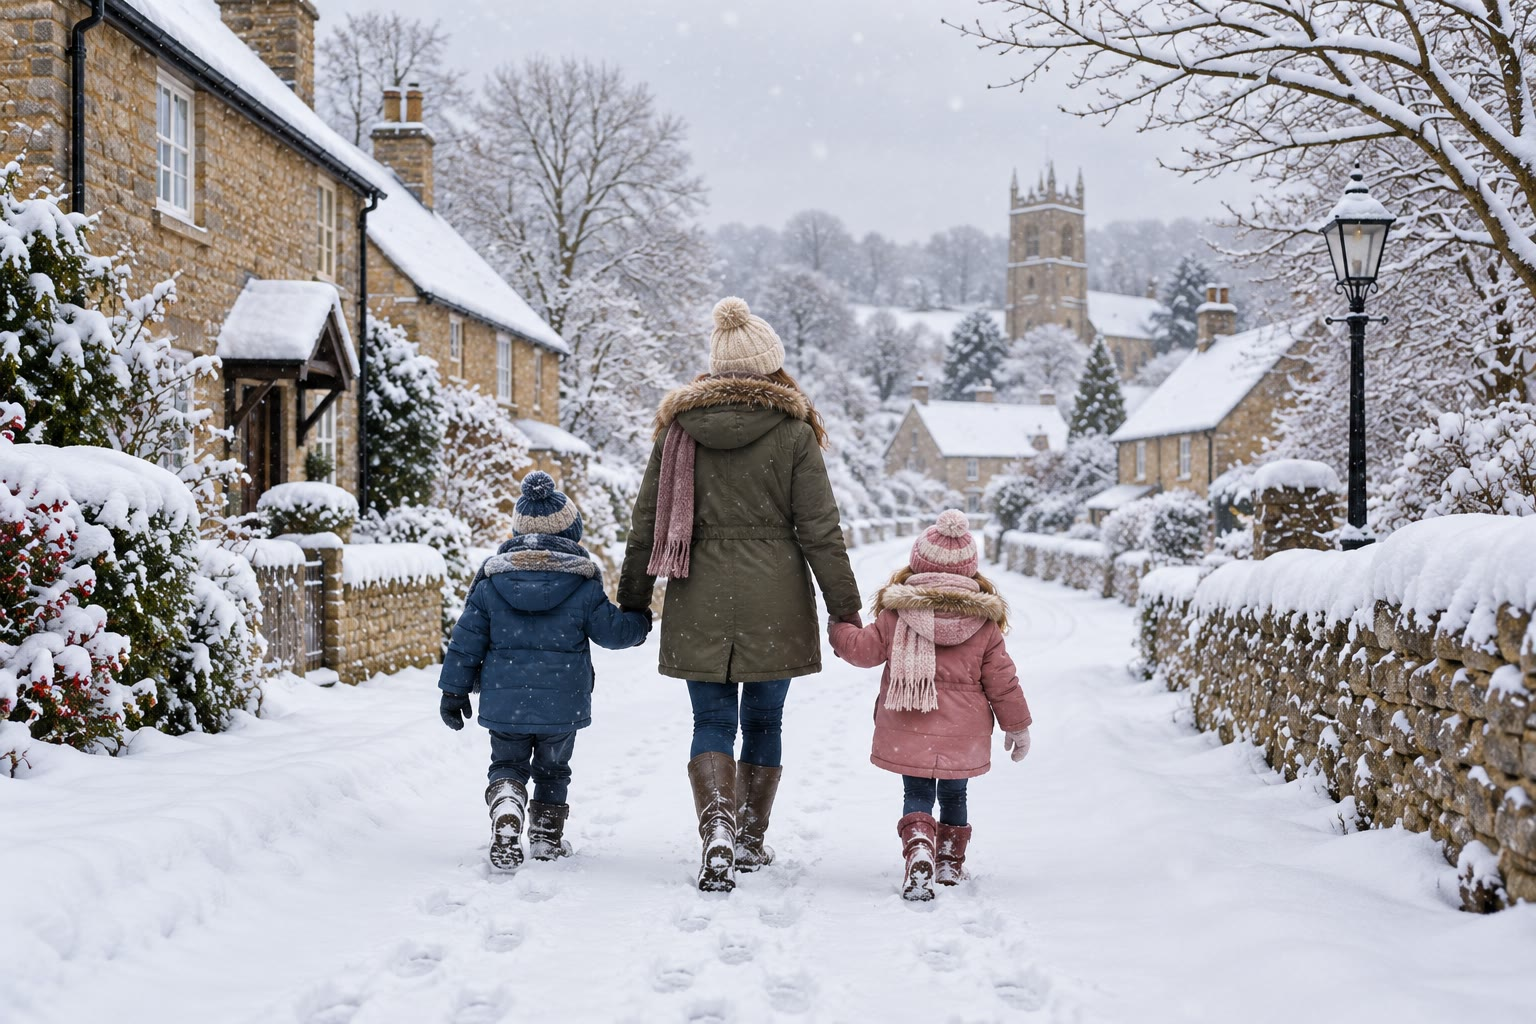
\includegraphics[width=\linewidth]{images/book1/ai/g1-snowy-street.jpg}

{\small De la neige, et il fait froid.}
\end{minipage}

\medskip
\begin{minipage}[b]{0.49\linewidth}\centering
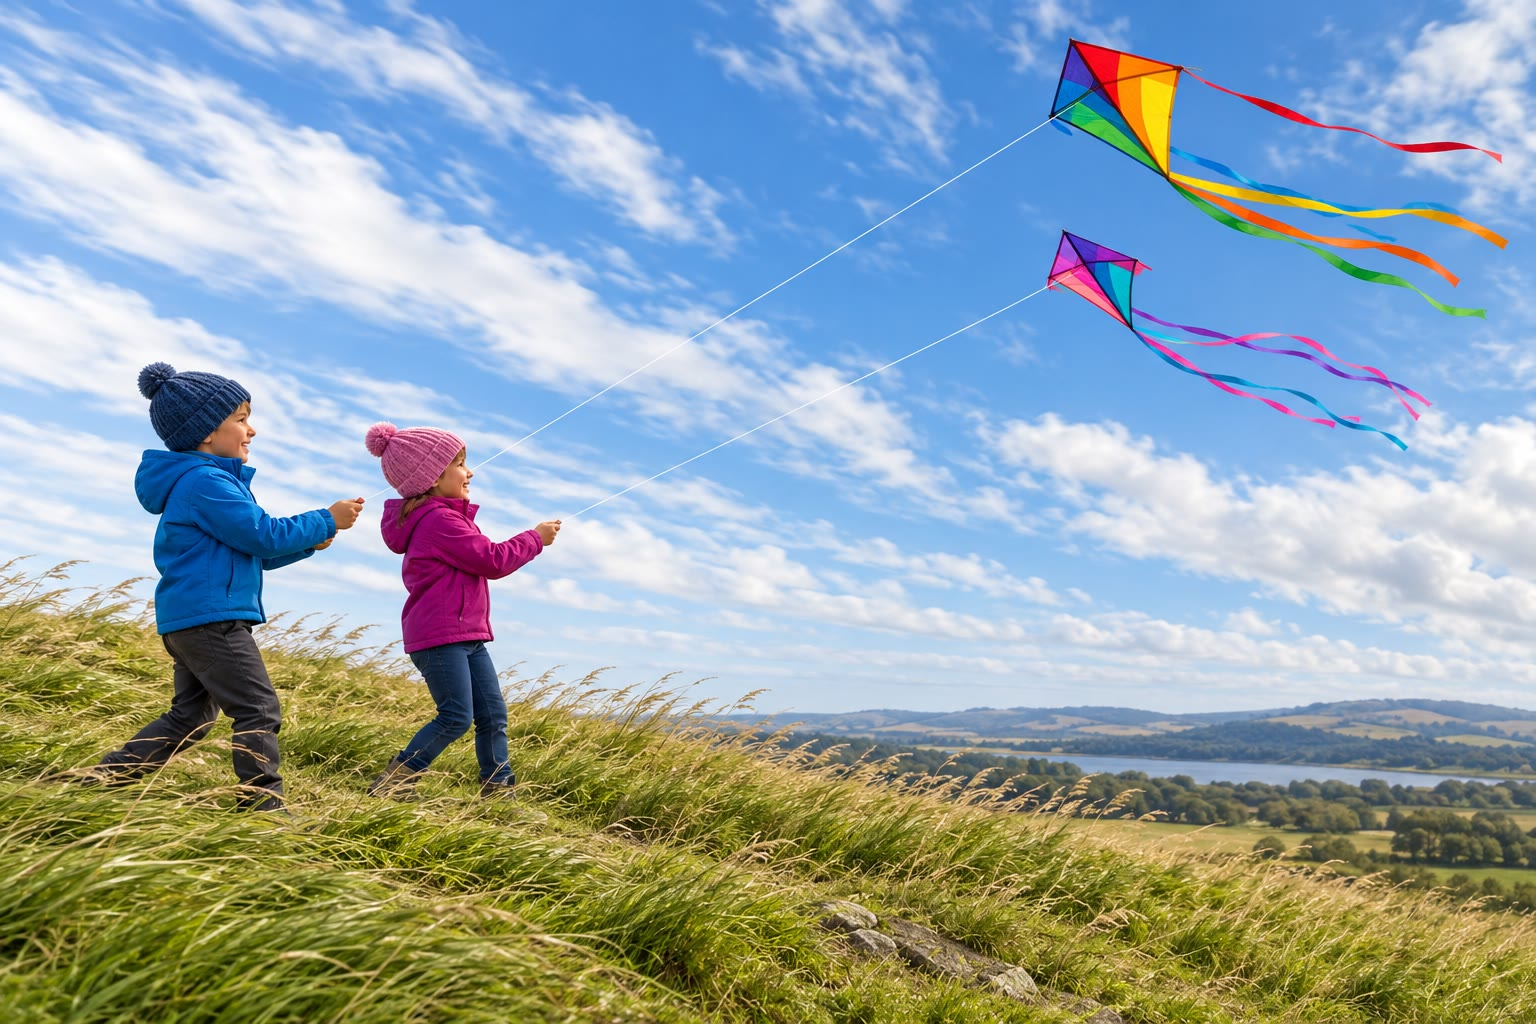
\includegraphics[width=\linewidth]{images/book1/ai/g1-windy-kites.jpg}

{\small Du vent~: les cerfs-volants volent.}
\end{minipage}\hfill
\begin{minipage}[b]{0.49\linewidth}\centering
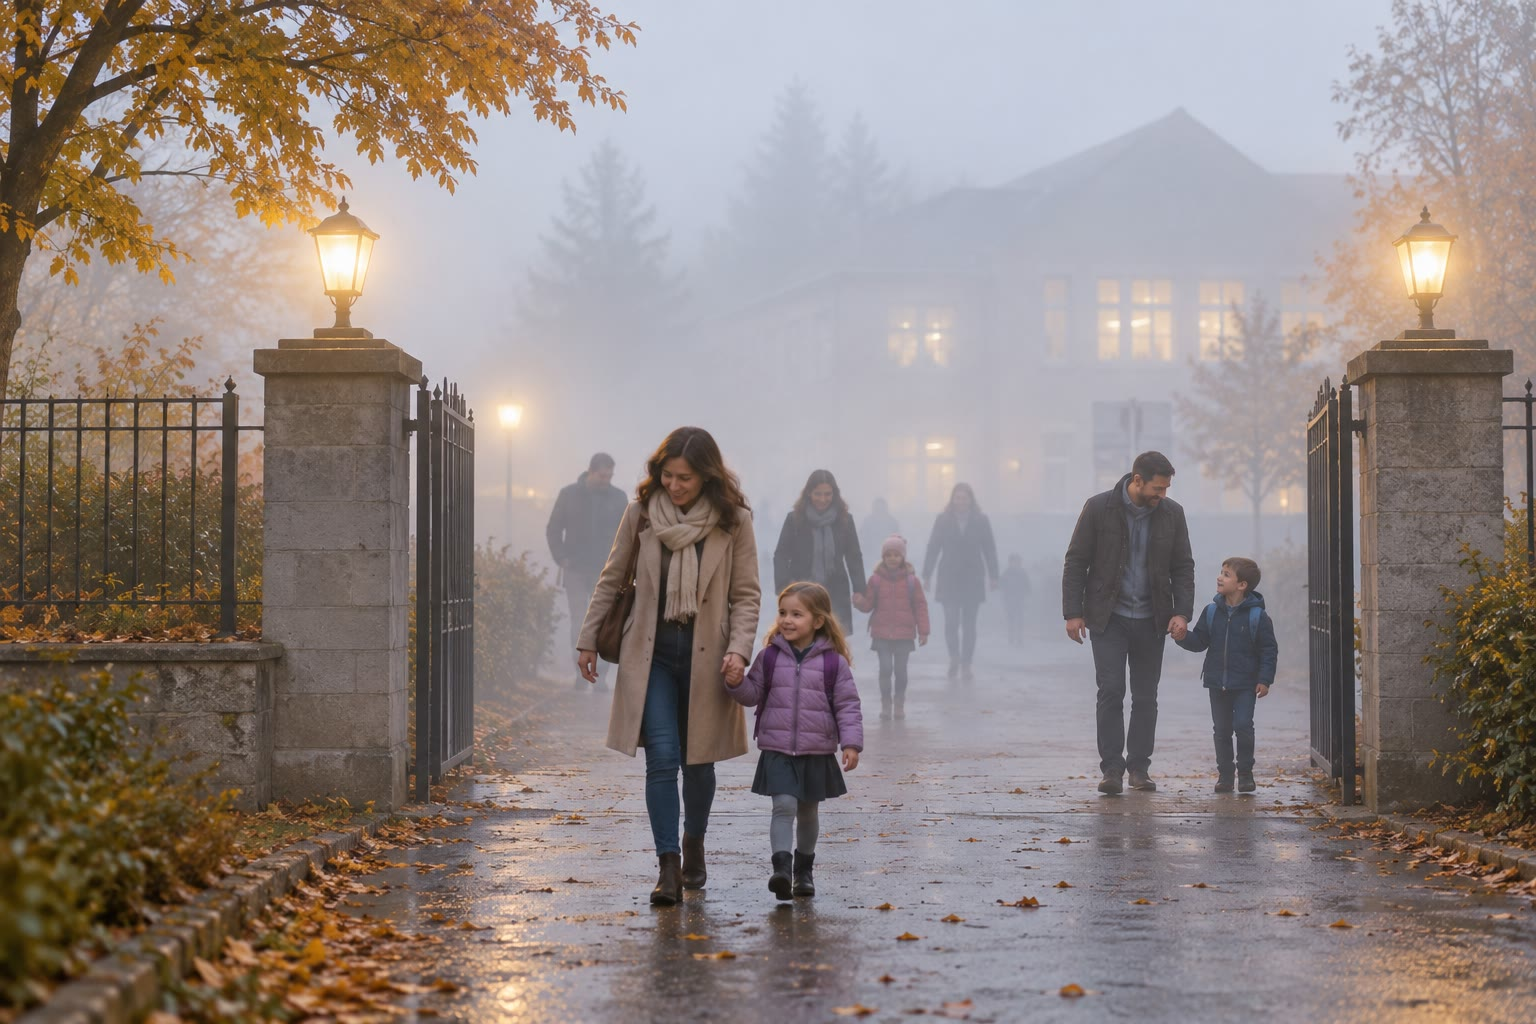
\includegraphics[width=\linewidth]{images/book1/ai/g1-foggy-school.jpg}

{\small Du brouillard~: on ne voit pas loin.}
\end{minipage}
\end{omfigure}

\begin{example}[Le brouillard]\label{ex:g1:watching-the-weather:fog}
Certains matins, l'air lui-même paraît blanc, et les arbres au bout de la
rue semblent disparaître. C'est le brouillard. Le brouillard est un nuage
qui touche le sol. Quand la journée se réchauffe, le brouillard s'en va souvent.
\end{example}

\section{Les symboles météo et le tableau météo}

Décrire le temps avec des mots prend du temps. Les personnes qui observent
le temps utilisent plutôt de petits dessins~: les \omterm{def:g1:watching-the-weather:weather-chart}{symboles météo}. Chaque
symbole est facile à dessiner et facile à reconnaître.

\begin{omfigure}
\begin{tikzpicture}[x=1cm, y=1cm]
  \foreach \i/\n/\t in {0/sun/soleil, 1/suncloud/soleil et nuages,
      2/cloud/nuages, 3/rain/pluie, 4/shower/averses} {
    \pic[scale=1.25, transform shape] at (\i*2.6,0) {omwx=\n};
    \node[font=\small, align=center, text width=2.4cm] at (\i*2.6,-1.05) {\t};
  }
  \foreach \i/\n/\t in {0/snow/neige, 1/storm/orage, 2/fog/brouillard,
      3/wind/vent} {
    \pic[scale=1.25, transform shape] at (\i*2.6+1.3,-2.6) {omwx=\n};
    \node[font=\small, align=center, text width=2.4cm] at (\i*2.6+1.3,-3.65) {\t};
  }
\end{tikzpicture}

{\small Neuf \omterm{def:g1:watching-the-weather:weather-chart}{symboles météo}. L'orage a un nuage sombre et un éclair~; les
averses arrivent avec des éclaircies entre elles.}
\end{omfigure}

\begin{definition}[Tableau météo]\label{def:g1:watching-the-weather:weather-chart}
Un \emph{symbole météo}\index{symbole météo} est un petit dessin qui montre
une sorte de temps. Un \emph{tableau météo}\index{tableau météo} est un
tableau dans lequel nous notons, jour après jour, le temps que nous avons
observé, à l'aide des symboles \omterm{def:g1:watching-the-weather:weather}{météo}.
\end{definition}

Une classe peut tenir un \omterm{def:g1:watching-the-weather:weather-chart}{tableau météo} pendant toute une semaine. Chaque
matin, et de nouveau chaque après-midi, un enfant regarde dehors et dessine
le symbole dans la bonne case. Nous notons aussi s'il fait chaud ou froid.

\begin{omfigure}
\begin{tikzpicture}[x=1cm, y=1cm]
  \def\cw{1.9}
  \foreach \d [count=\i from 0] in {Lundi, Mardi, Mercredi, Jeudi,
      Vendredi, Samedi, Dimanche}
    \node[font=\scriptsize\bfseries] at ({1.6+\i*\cw+\cw/2},0.35) {\d};
  \node[font=\scriptsize\bfseries, anchor=east] at (1.45,-0.5) {matin};
  \node[font=\scriptsize\bfseries, anchor=east] at (1.45,-1.5) {après-midi};
  \node[font=\scriptsize\bfseries, anchor=east, align=right] at (1.45,-2.35) {chaud ou\\froid~?};
  \draw[black!60] (1.6,0) rectangle ({1.6+7*\cw},-2.7);
  \foreach \i in {1,...,6}
    \draw[black!60] ({1.6+\i*\cw},0.65) -- ({1.6+\i*\cw},-2.7);
  \draw[black!60] (1.6,0.65) -- ({1.6+7*\cw},0.65);
  \draw[black!60] (1.6,0.65) -- (1.6,0);
  \draw[black!60] ({1.6+7*\cw},0.65) -- ({1.6+7*\cw},0);
  \draw[black!60] (1.6,-1) -- ({1.6+7*\cw},-1);
  \draw[black!60] (1.6,-2) -- ({1.6+7*\cw},-2);
  \foreach \i/\m/\a/\w in {0/rain/rain/froid, 1/cloud/suncloud/froid,
      2/sun/sun/chaud, 3/sun/suncloud/chaud, 4/suncloud/shower/chaud,
      5/fog/sun/chaud, 6/cloud/rain/froid} {
    \pic[scale=0.8, transform shape] at ({1.6+\i*\cw+\cw/2},-0.5) {omwx=\m};
    \pic[scale=0.8, transform shape] at ({1.6+\i*\cw+\cw/2},-1.5) {omwx=\a};
    \node[font=\scriptsize] at ({1.6+\i*\cw+\cw/2},-2.35) {\w};
  }
\end{tikzpicture}

{\small Le \omterm{def:g1:watching-the-weather:weather-chart}{tableau météo} tenu par une classe pendant une semaine de printemps.}
\label{fig:g1:watching-the-weather:chart}
\end{omfigure}

\begin{method}[Lire un tableau météo]\label{met:g1:watching-the-weather:read}
Pour lire un \omterm{def:g1:watching-the-weather:weather-chart}{tableau météo}~:
\begin{enumerate}
  \item trouve la colonne du jour que tu cherches~;
  \item regarde la ligne~: le matin, ou l'après-midi~;
  \item dis quel temps montre le symbole.
\end{enumerate}
Pour savoir combien de jours il y a eu du soleil, fais glisser ton doigt le
long d'une ligne et compte les symboles du soleil.
\end{method}

\begin{example}[Lire le tableau de la classe]\label{ex:g1:watching-the-weather:read}
Sur le tableau de cette classe, lundi matin, il pleuvait et il faisait
froid. Mercredi, il y a eu du soleil toute la journée. Samedi, le
brouillard du matin a laissé place au soleil l'après-midi. Les matins de la
semaine, la classe a dessiné le soleil 2 jours~: mercredi et jeudi.
\end{example}

\section{Le temps change}

Le temps ne reste pas le même. Il change pendant la journée, d'un jour à
l'autre, et au fil de l'année.

\begin{itemize}
  \item \textbf{Pendant une journée.} Un matin gris peut se changer en un
        après-midi ensoleillé. Un matin d'un bleu limpide peut finir par un
        orage. Tôt le matin et la nuit, il fait en général plus frais que
        l'après-midi.
  \item \textbf{D'un jour à l'autre.} Regarde le tableau de la classe~:
        aucun jour de la semaine ne ressemble tout à fait à un autre.
  \item \textbf{Au fil de l'année.} En été, les journées sont en général
        chaudes, et en hiver, elles sont en général froides~; dans beaucoup
        d'endroits, la neige ne tombe qu'en hiver. Les livres de physique
        expliquent pourquoi les saisons reviennent chaque année.
\end{itemize}

\begin{omfigure}
\begin{tikzpicture}[x=1cm, y=1cm]
  \draw[black!50, line width=0.8pt, -{Stealth[length=2.5mm]}] (0,0) -- (12.2,0);
  \foreach \x/\n/\t/\h in {0.9/fog/tôt le matin/frais, 3.5/suncloud/matin/doux,
      6.1/sun/après-midi/chaud, 8.7/storm/fin d'après-midi/chaud et orageux,
      11.2/suncloud/soir/plus frais} {
    \pic[scale=1.1, transform shape] at (\x,0.85) {omwx=\n};
    \fill[black!60] (\x,0) circle (1.5pt);
    \node[font=\scriptsize\bfseries, below] at (\x,-0.12) {\t};
    \node[font=\scriptsize, below] at (\x,-0.5) {\h};
  }
\end{tikzpicture}

{\small Une journée d'été, du matin au soir~: le temps change cinq
fois.}
\label{fig:g1:watching-the-weather:day}
\end{omfigure}

\begin{omfigure}
\begin{tikzpicture}[x=1cm, y=1cm]
  \foreach \i/\s/\c/\g/\w/\gr in {0/printemps/green!55!black/pink!60/suncloud/green!35,
      1/été/green!45!black/green!50!black/sun/green!35,
      2/automne/orange!80!black/orange!70/rain/green!25!brown!30,
      3/hiver/black!55/white/snow/white} {
    \begin{scope}[shift={(\i*3.15,0)}]
      \draw[black!30, rounded corners=3pt, fill=ocBlue!6] (-1.4,-0.45) rectangle (1.4,3.05);
      \fill[\gr] (-1.4,-0.45) rectangle (1.4,0);
      \draw[black!25] (-1.4,0) -- (1.4,0);
      \fill[brown!60!black] (-0.09,0) rectangle (0.09,1.0);
      \draw[brown!60!black, line width=1.6pt] (0,0.75) -- (-0.5,1.35);
      \draw[brown!60!black, line width=1.6pt] (0,0.9) -- (0.45,1.45);
      \ifnum\i<3
        \fill[\c, opacity=0.85] (0,1.55) circle (0.72);
        \ifnum\i=0 \foreach \a in {20,80,140,200,260,320} \fill[\g] (0,1.55) ++(\a:0.45) circle (0.09); \fi
        \ifnum\i=2 \foreach \x/\y in {-0.9/0.15,0.7/0.3,0.95/0.1} \fill[\g] (\x,\y) circle (0.07); \fi
      \else
        \draw[white, line width=2.4pt] (-0.5,1.35) -- (-0.35,1.17);
        \draw[white, line width=2.4pt] (0.45,1.45) -- (0.3,1.27);
      \fi
      \pic[scale=0.8, transform shape] at (0.95,2.55) {omwx=\w};
      \node[font=\small\bfseries] at (0,-0.75) {\s};
    \end{scope}
  }
\end{tikzpicture}

{\small Le même arbre au fil des quatre saisons~: en fleurs au printemps,
couvert d'épaisses feuilles vertes en été, perdant ses feuilles orange en
automne, les branches nues sous la neige en hiver.}
\label{fig:g1:watching-the-weather:seasons}
\end{omfigure}

\begin{remark}[D'où vient le vent]\label{rem:g1:watching-the-weather:wind}
Nous ne pouvons pas voir le vent, mais nous pouvons voir ce qu'il fait. Un
drapeau, une manche à air ou la fumée d'une cheminée sont poussés par le
vent~: ils montrent où va le vent, donc le vent vient de l'autre côté.
\end{remark}

\begin{omfigure}
\begin{tikzpicture}[x=1cm, y=1cm]
  % ground
  \fill[green!30!omLithAlluv] (-0.4,-0.1) rectangle (8.4,0);
  % windsock on a pole
  \draw[black!70, line width=1.2pt] (1,0) -- (1,3.2);
  \fill[orange!85, draw=black!60] (1,3.15) -- (3.4,2.95) -- (3.4,2.55) -- (1,2.45) -- cycle;
  \fill[white] (1.6,3.1) -- (2.2,3.05) -- (2.2,2.5) -- (1.6,2.47) -- cycle;
  \fill[white] (2.8,3.0) -- (3.4,2.95) -- (3.4,2.55) -- (2.8,2.53) -- cycle;
  \draw[black!60] (1,3.15) -- (3.4,2.95) -- (3.4,2.55) -- (1,2.45);
  % flag
  \draw[black!70, line width=1.2pt] (5.4,0) -- (5.4,3.2);
  \fill[ocBlue!70, draw=black!60] (5.4,3.15) .. controls (6.0,3.3) and (6.4,2.9) .. (7.1,3.05)
     -- (7.1,2.35) .. controls (6.4,2.2) and (6.0,2.6) .. (5.4,2.45) -- cycle;
  % wind arrows
  \foreach \y in {1.0,1.6}
    \draw[omWxRain, line width=1.4pt, -{Stealth[length=3mm]}] (-0.3,\y) -- (0.7,\y);
  \node[font=\small, align=right, anchor=east] at (-0.45,1.3) {le vent\\vient d'ici};
  \draw[black!60, -{Stealth[length=2mm]}] (4.1,2.75) -- (4.9,2.75);
  \node[font=\small, align=left, anchor=west] at (7.5,2.7) {le drapeau et la\\manche à air\\montrent où\\va le vent};
\end{tikzpicture}

{\small Une manche à air et un drapeau, un jour de vent. Le vent souffle de
la gauche vers la droite.}
\end{omfigure}

\section{Pourquoi observer le temps~?}

Beaucoup de gens ont besoin de savoir quel temps il va faire.
\begin{itemize}
  \item \textbf{Les agriculteurs} regardent le ciel avant de couper le
        foin~: la pluie le gâterait. Au printemps, ils redoutent une nuit
        de gel qui pourrait tuer les jeunes plantes.
  \item \textbf{Les marins et les pêcheurs} surveillent le vent~: un vent
        fort lève de grosses vagues, et les bateaux restent au port.
  \item \textbf{Les pilotes} doivent tout savoir du brouillard, des
        orages et du vent avant qu'un avion décolle.
  \item \textbf{Une classe} qui part en sortie en forêt veut savoir s'il
        faut emporter des imperméables ou des chapeaux de soleil.
\end{itemize}
Chaque jour, des personnes appelées météorologues observent le temps dans
le monde entier et nous disent, à la radio, à la télévision ou sur un
téléphone, quel temps il fera probablement les jours suivants.

\begin{example}[Les signes du ciel]\label{ex:g1:watching-the-weather:signs}
Bien avant la radio et les téléphones, les gens ont appris à lire le ciel.
Quand de petits nuages blancs grandissent, l'après-midi, jusqu'à devenir de
hautes tours sombres, une averse ou un orage approche. Quand le vent tourne
et que le ciel se couvre lentement d'un voile gris, la pluie arrive souvent
quelques heures plus tard. Ces signes ne disent pas toujours vrai, mais ils
sont souvent utiles.
\end{example}

\section{S'habiller selon le temps}

Maintenant, Lena peut répondre à sa question. Il pleut et il fait froid,
donc elle mettra son imperméable et ses bottes. Demain, le temps sera
peut-être différent, et elle choisira de nouveau.

\begin{omfigure}
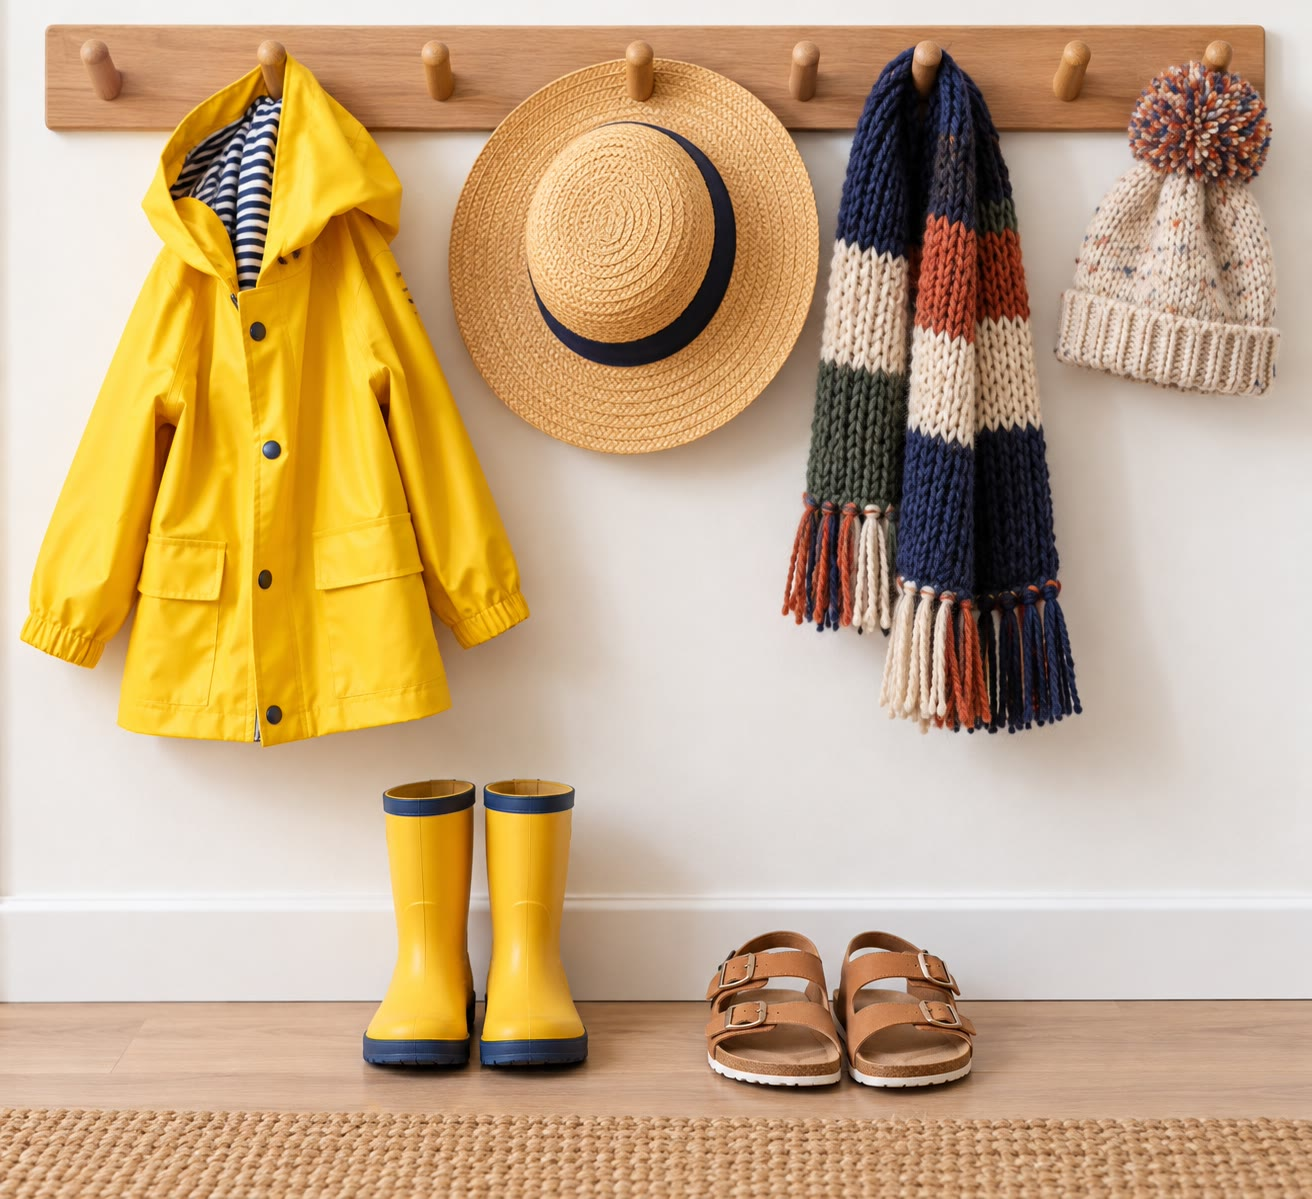
\includegraphics[width=0.66\linewidth]{images/book1/ai/g1-coat-pegs.jpg}

{\small Des vêtements pour chaque sorte de temps~: un imperméable, un
chapeau de soleil, une écharpe et un bonnet, des bottes et des sandales.}
\end{omfigure}

\begin{method}[Choisir ses vêtements selon le temps]\label{met:g1:watching-the-weather:clothes}
Regarde le ciel et sens l'air, puis~:
\begin{itemize}
  \item pluie ou averses~: un imperméable ou un parapluie, et des bottes~;
  \item froid ou neige~: un blouson chaud, une écharpe, un bonnet et des gants~;
  \item grand soleil et chaleur~: un chapeau de soleil, des vêtements
        légers, et de l'eau à boire~;
  \item vent~: un blouson qui ferme bien~; un parapluie n'aide pas beaucoup.
\end{itemize}
\end{method}

\begin{safety}
\textbf{Ne regarde jamais le Soleil en face}, pas même un instant, et
jamais à travers des lunettes, des jumelles ou un appareil photo~: tes
yeux pourraient être abîmés pour toujours. Pendant un orage, reste à
l'intérieur ou dans une voiture, éloigne-toi des grands arbres et de l'eau,
et attends que l'orage soit passé.
\end{safety}

\section{Exercices}

\begin{exercise}[$\star$]\label{exo:g1:watching-the-weather:1}
Dessine le symbole de chaque temps~: soleil~; pluie~; neige~; nuages.
\end{exercise}

\begin{exercise}[$\star$]\label{exo:g1:watching-the-weather:2}
Quel temps fait-il sur chacune des quatre images de la section
«~Quel temps fait-il~?~»~? Réponds en un ou deux mots pour chacune.
\end{exercise}

\begin{exercise}[$\star$]\label{exo:g1:watching-the-weather:3}
Regarde le \omterm{def:g1:watching-the-weather:weather-chart}{tableau météo} de la classe. Quel temps faisait-il mardi matin~?
Vendredi après-midi~? Dimanche après-midi~?
\end{exercise}

\begin{exercise}[$\star$]\label{exo:g1:watching-the-weather:4}
Sur le \omterm{def:g1:watching-the-weather:weather-chart}{tableau météo} de la classe, quel jour y a-t-il eu du soleil le matin
et l'après-midi~?
\end{exercise}

\begin{exercise}[$\star$]\label{exo:g1:watching-the-weather:5}
Associe chaque vêtement à un temps~: un chapeau de soleil~; des bottes et un
imperméable~; une écharpe et des gants. Les temps sont~: froid avec de la
neige~; chaud avec du soleil~; pluvieux.
\end{exercise}

\begin{exercise}[$\star$]\label{exo:g1:watching-the-weather:6}
Lena dit~: «~Regarde, le drapeau claque~!~» Quel temps fait-il~?
\end{exercise}

\begin{exercise}[$\star$]\label{exo:g1:watching-the-weather:7}
Vrai ou faux~? Explique.
\begin{enumerate}
  \item Le temps est toujours le même le matin et l'après-midi.
  \item Le brouillard est un nuage qui touche le sol.
  \item La règle «~ne jamais regarder le Soleil, même d'un seul œil~» est une bonne règle.
\end{enumerate}
\end{exercise}

\begin{exercise}[$\star\star$]\label{exo:g1:watching-the-weather:8}
Sur le \omterm{def:g1:watching-the-weather:weather-chart}{tableau météo} de la classe, compte les après-midi avec de la pluie
ou des averses. Compte les jours froids. La semaine a-t-elle été plutôt
chaude ou plutôt froide~?
\end{exercise}

\begin{exercise}[$\star\star$]\label{exo:g1:watching-the-weather:9}
Voici ce que Sam a vu de sa fenêtre pendant une journée~: le matin, un ciel
gris~; à midi, des gouttes sur la vitre~; le soir, un ciel bleu avec
quelques nuages. Dessine les trois \omterm{def:g1:watching-the-weather:weather-chart}{symboles météo} dans le bon ordre.
\end{exercise}

\begin{exercise}[$\star\star$]\label{exo:g1:watching-the-weather:10}
Sur l'image de la manche à air et du drapeau, le vent vient de la gauche.
Un autre jour, un drapeau montre la gauche. De quel côté vient le vent ce
jour-là~?
\end{exercise}

\begin{exercise}[$\star\star$]\label{exo:g1:watching-the-weather:11}
Regarde le dessin du même arbre au fil des quatre saisons. En quelle saison
l'arbre n'a-t-il pas de feuilles~? En quelle saison est-il en fleurs~?
Quel \omterm{def:g1:watching-the-weather:weather-chart}{symbole météo} est dessiné pour l'hiver, et pourquoi va-t-il bien avec
cette saison~?
\end{exercise}
